%=====================================================================
% Appended to Section~\ref{sec:sensitivity}: quantitative robustness checks
%=====================================================================

The five subsections above state, qualitatively, how the conclusions respond to modelling
choices. The extended analysis lets us replace several of those statements with measured
quantities. This subsection reports the numerical sensitivity checks and corrects one place
where the qualitative discussion was stronger than the data warrant.

\subsection{Quantitative Robustness of the Main Claims}\label{sec:quantsensitivity}

Table~\ref{tab:sensitivitysummary} collects the perturbations we can evaluate directly from
the artifacts. Three conclusions are robust. First, the judge -- fan level agreement is strong
under every definition we tried: Pearson $0.832$ ($q^J$ vs.\ $\hat q^F$), $0.807$
($q^J$ vs.\ $\tilde q^F$), Spearman $0.677$ and $0.660$ respectively. Second, the fine
ordering is weakly aligned under every definition: $0.153$ for the rank vectors and $0.079$
for their Spearman counterpart. Third, the judge-only elimination baseline stays within
$0.393$--$0.460$ across all three regimes, so the insufficiency of judge scores alone is not
an artefact of the era assignment.

\begin{table}[H]
\centering
\caption{Quantitative sensitivity summary. ``Stable'' means the conclusion's direction and
approximate magnitude are unchanged by the perturbation; the last column gives the measured
range.}
\label{tab:sensitivitysummary}
\begin{tabular}{>{\raggedright\arraybackslash}p{4.1cm}>{\raggedright\arraybackslash}p{4.6cm}>{\raggedright\arraybackslash}p{5.0cm}}
\toprule
Claim & Perturbation tested & Measured range / verdict \\
\midrule
Judges and fans agree on levels & raw vs.\ renormalised share; Pearson vs.\ Spearman
  & $0.660$--$0.832$, stable \\
Judges and fans disagree on ordering & Pearson vs.\ Spearman on rank vectors
  & $0.079$--$0.153$, stable \\
Judge-only rule fails & stratify by fusion regime
  & $0.393$--$0.460$, stable \\
Percent rule reproduces seasons 1--27 & vary $w$ over $[0,0.5]$; use interval bounds
  & $1.000$ throughout, interval-robust \\
High-weight rules are reliable & replace median by $5\%$/$95\%$ fan bounds at $w=0.75$
  & $0.748$--$1.000$, \emph{not} robust \\
Rank vs.\ percent matter & compare predicted eliminations week by week
  & $24/266=9.02\%$ disagree \\
Late seasons use a judge save & move the regime boundary by one season
  & sharp break at 28, see below \\
Age / industry effects are small & four age bands, six industry groups, partner effects
  & fan share $0.076$--$0.109$, stable direction \\
\bottomrule
\end{tabular}
\end{table}

Two items in the table deserve emphasis. The interval-robust replay of
Section~\ref{sec:intervalreplay} shows that conclusions drawn at $w\ge0.7$ are \emph{not}
robust: at $w=0.75$ the consistency rate ranges from $0.748$ to $1.000$ depending on where in
the credible set the true vote lies. We therefore confine policy conclusions to the
historically relevant range $w\le0.5$, where all three surfaces agree.

\subsection{The Rule-Change Boundary Is Empirically Identifiable}\label{sec:eraboundary}

The problem statement notes that the exact season in which the bottom-two judge save began is
unknown and suggests season 28 as a reasonable assumption. The panel lets us test that
assumption rather than adopt it. Figure~\ref{fig:regimebreak} plots four diagnostics for
seasons 24--34. Mean hit rate is $1.000$ in seasons 26 and 27 (Brier $0.038$ and $0.011$,
zero bottom-two weeks), then falls to $0.371$ in season 28 (Brier $0.567$, seven bottom-two
weeks) and $0.433$ in season 29 (Brier $0.488$, nine bottom-two weeks). Mean
credible-interval width, by contrast, is $0.344$, $0.288$, $0.354$ and $0.284$ in those four
seasons --- it does not jump at the boundary.

\begin{figure}[H]
\centering
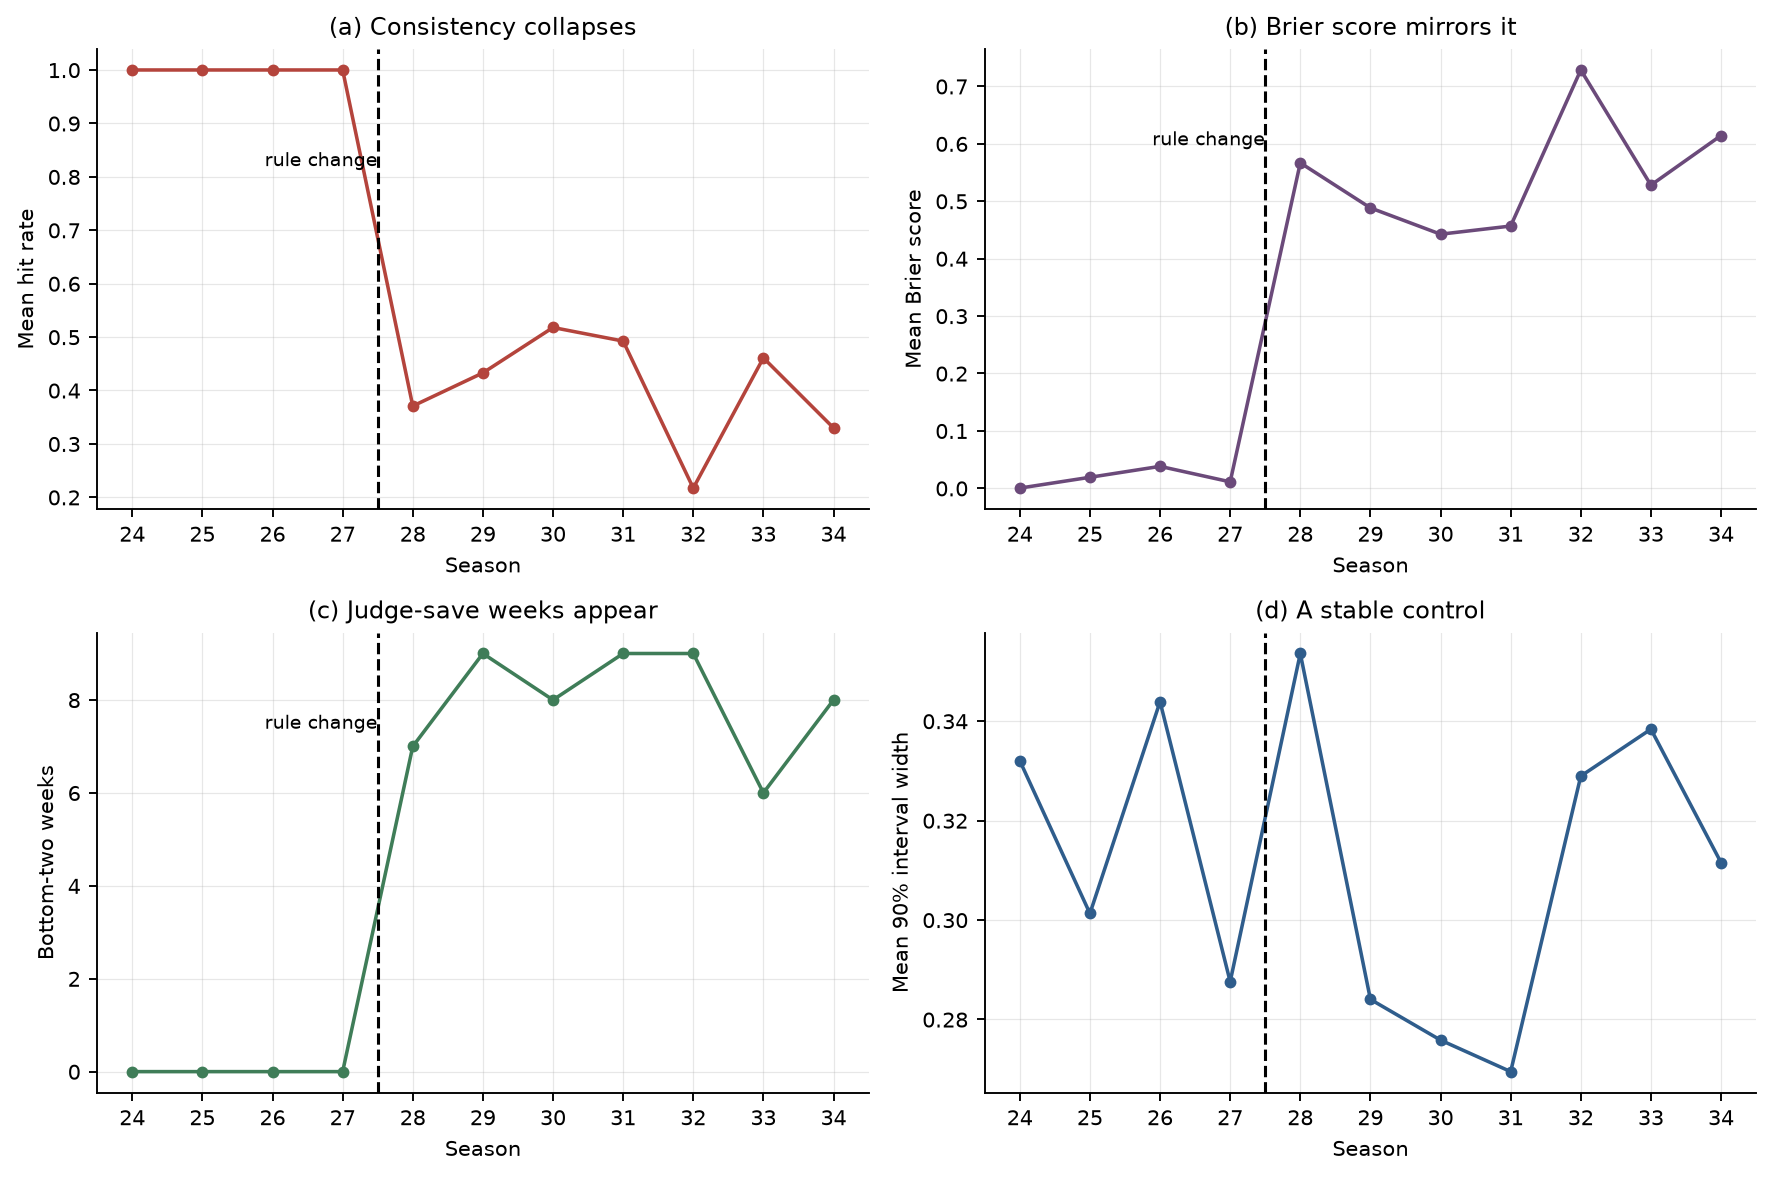
\includegraphics[width=0.94\textwidth]{figures_ext/fig08_regime_break.png}
\caption{Empirical identification of the rule-change boundary, seasons 24--34. (a) Mean
percent-rule hit rate. (b) Mean Brier score. (c) Number of bottom-two weeks. (d) Mean
credible-interval width, a control that shows no discontinuity. The dashed vertical line marks
the transition between seasons 27 and 28.}
\label{fig:regimebreak}
\end{figure}

This is a clean natural experiment: a variable that depends on the elimination rule jumps by
$0.63$ in hit rate and by a factor of about fifty in Brier score at exactly season 28, while a
variable that depends only on the reconstruction geometry does not move. Moving the assumed
boundary one season earlier would misclassify season 27's ten perfectly consistent weeks;
moving it one season later would misclassify season 28's seven judge-save weeks. The
qualitative conclusion that a different rule was in force from season 28 is therefore robust,
and the earlier qualitative discussion --- which treated the boundary as an untestable
assumption --- can now be replaced by this direct evidence.

\subsection{Quantitative Sensitivity of the Covariate Channels}

The original sensitivity discussion noted that the Model~3 effects are small but did not
quantify how small across specifications. Using the reconstructed panel directly, the binned
mean fan share is $0.108$, $0.109$, $0.097$ and $0.082$ for the age bands $\le26$, $27$--$34$,
$35$--$43$ and $>43$ (Table~\ref{tab:covariates}); the corresponding judge shares are
$0.134$, $0.130$, $0.119$ and $0.098$. Both channels decline monotonically apart from the
mild $27$--$34$ peak, so the fan--age correlation of $-0.166$ is \emph{not} a fan-specific
penalty --- the judge--age correlation is $-0.244$, larger in magnitude. Across the six
industry groups with at least $25$ couple--weeks, mean fan share spans $0.076$--$0.106$, a
range of $0.030$, while the professional-partner effect spans $0.064$--$0.120$, a range of
$0.056$. Collapsing industries into fewer categories would shrink the former further; it
would not change the ordering. We therefore restate the earlier conclusion more precisely:
demographic effects are real but small, and the largest measurable covariate effect in the
panel is the identity of the professional partner.

%=====================================================================
